In this section the results of this project are shown.

\subsection{Communication}
In this section the results are shown with respect to the inter-node communication. As mentioned in section \ref{med:comm} the benchmark is communication heavy and this might influence the performance. With the following results we would like to get feel for the amount of time is spent sending messages.

\subsubsection{IMB benchmark}
On each of the systems, we have used the IMB benchmark has been done. To find the time it takes to send messages between two machines. The communications which are relevant are 0, 1028 and 2048 bytes. The 0-bytes times shows the time it takes to send the FINISH message as mentioned in section \ref{med:comm}, 1028 bytes gives an indication of how much time it will take to send a message without a completely full buffer, and lastly the 2048 shows the time it takes to send a full buffer. The complete table is shown in Appendix [REF to appendix].
\begin{table}[!h]
\begin{tabular}{|l|l|l|l|l|}
\hline
Bytes & DAS-4 ($\mu sec$) & DAS-4 no InfiniBand($\mu sec$) & OpenNebula ($\mu sec$) & AWS EC2 ($\mu sec$)\\ \hline
0 & 3.81 &  46.55  & 112.75 &   81.82 \\ \hline
1024 & 4.93 & 56.97  &  130.76 &  91.40  \\ \hline 
2048 & 5.96 4 & 68.36 & 269.74 &  102.96 \\ \hline
4096 & 7.36 & 79.08  & 344.64 &  125.58  \\ \hline 
\end{tabular}
\caption{This figure shows the IMB benchmarks on the different platforms used. All times are an average of a 1000 messages sent. Only the relevant sizes have been shown.}
\label{tab:imb_bench}
\end{table}

\subsubsection{Message count}
The message count is an important number to calculate the communication time. The amount of data which is sent per message can be estimated. By using this estimation the number of messages can be calculated. As mentioned before in \cite{suzumura2011performance}, an estimation of the amount of bytes is computed using \ref{eq:communication_size}. The figure \ref{fig:das_scale_messages} shows the computed and the observed amount of messages sent per node ,as a function of the scale. The bars named comp show the computed number of messages and obs show the observed number of messages. Figure \ref{fig:scale_messages} shows that the observed number of messages is much lower than the calculated number. By multiplying the number of observed messages by 2 figure \ref{fig:scale_messages_doubled} is created. The figure shows that is a factor two difference between the number of messages. 
\begin{figure}[!h]
\centering
\begin{subfigure}{.5\textwidth}
  \centering
  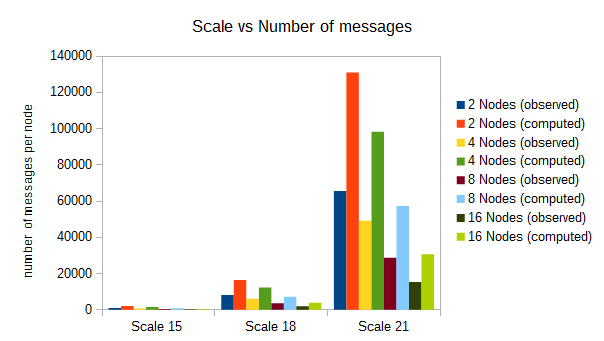
\includegraphics[width=\linewidth]{images/scale_vs_messages.png}
  \caption{The number of messages as a function of scale for different number of nodes.}
  \label{fig:scale_messages}
\end{subfigure}%
\begin{subfigure}{.5\textwidth}
  \centering
  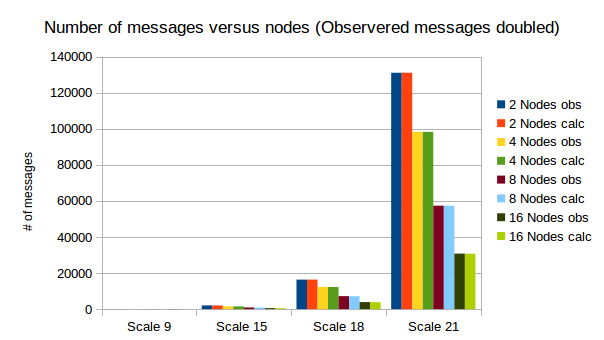
\includegraphics[width=\linewidth]{images/scale_vs_messages_doubled.png}
  \caption{The same graph as figure \ref{fig:scale_messages}, but with the observed number of messages doubled}
  \label{fig:scale_messages_doubled}
\end{subfigure}
\caption{The number of messages sent per node for 4 different scales and 2 to 16 nodes. The observed number is the number of messages sent per node when the buffer is full + the messages send with left overs(see section \ref{med:comm})}
\label{fig:das_scale_messages}
\end{figure}


\subsection{OpenMP}
\label{sec:openmp}
In figure \ref{fig:openmp_scale_cpu} we present the results from the OpenMP experiments. 
The figure shows that the performance of the modified \texttt{graph500\_mpi\_simple} does not depend on the number of nodes used. This does not change as the scale of the problem increases as figure \ref{fig:openmp_scale}. The performance is not dependent on the number of CPUs. This was an unexpected result and means that OpenMP is not used during the BFS.

\begin{figure}[!h]
\centering
\begin{subfigure}{.5\textwidth}
  \centering
  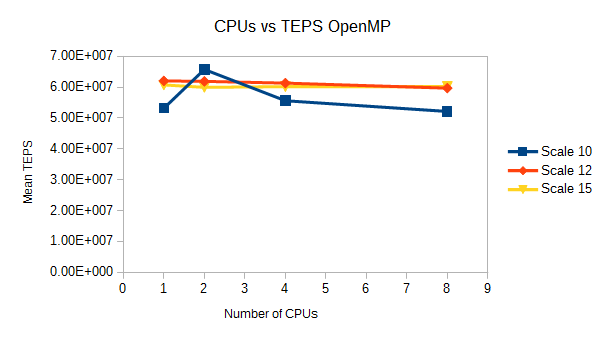
\includegraphics[width=\linewidth]{images/openmp_cpus.png}
  \caption{Against CPU}
  \label{fig:openmp_cpu}
\end{subfigure}%
\begin{subfigure}{.5\textwidth}
  \centering
  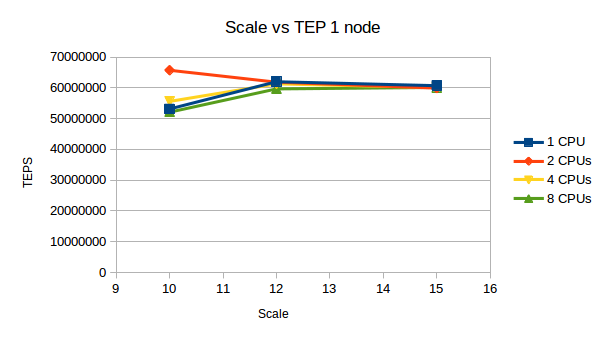
\includegraphics[width=\linewidth]{images/openmp_scale.png}
  \caption{Against scale}
  \label{fig:openmp_scale}
\end{subfigure}
\caption{The effect of different scales and the numbers of CPUs on the (TEPS)}
\label{fig:openmp_scale_cpu}
\end{figure}

\subsection{DAS-4}
In this section the results are shown for the experiments on DAS-4. Only experiments done in next section and in section \ref{sec:openmp} have been done with validation, all other experiments have been done without validation.

\subsubsection{Turning validation off}
\label{sec:noval}
 Figure \ref{fig:val_vs_noval} TEPS as a function of the scale (figure \ref{fig:scale_val_noval}) and the number of nodes (figure \ref{fig:nodes_val_noval}). The results show that there is a difference in the number of TEPS with and without the validation. The difference in performance can be up to 50\% in the case of scale 15 with 16 nodes. What can be noticed in figure \ref{fig:nodes_val_noval} is that the same trends are followed as the number of nodes increases.
 Figure \ref{fig:scale_no_val} shows that for larger scales the difference between the validation and non validation becomes larger.
The difference in performance does not differ too much and they show the behavior. This means that the estimation that is done using the no validation experiments are comparable to with validation. This is the expected result. 
 %TODO differences bereken tussen val en no validation.
\begin{figure}[!h]
\centering
\begin{subfigure}{.5\textwidth}
  \centering
  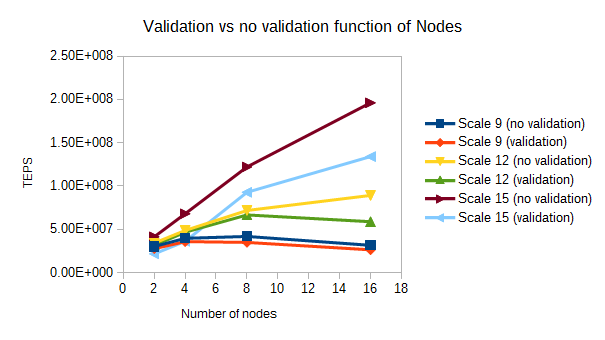
\includegraphics[width=\linewidth]{images/nodes_scale_vs_noscale.png}
  \caption{As a function of nodes}
  \label{fig:nodes_val_noval}
\end{subfigure}%
\begin{subfigure}{.5\textwidth}
  \centering
  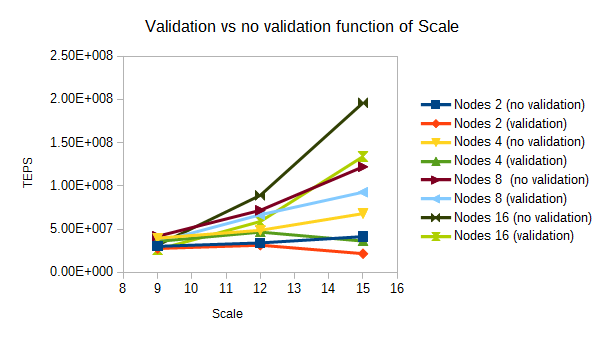
\includegraphics[width=\linewidth]{images/scale_val_vs_noval.png}
  \caption{As a function of scale}
  \label{fig:scale_val_noval}
\end{subfigure}
\caption{The effect of different scales and the numbers of CPUs on the TEPS between the program with and without validation.}
\label{fig:val_vs_noval}
\end{figure}

\subsubsection{Nodes and Scale}
\label{res:nodes_scale}
Figure \ref{fig:das_no_val} shows the amount of TEPS increases as the number of nodes increases. The larger the amount of nodes the more edges can be traversed, as seen in figure \ref{fig:scale_no_val}. This increase in TEPS can be seen up till a certain point. After this tipping point the amount of TEPS decreases again. The tipping point can be found for any number of nodes, although it the performance is almost constant for 2 and 4 nodes for each scale.
Figure \ref{fig:nodes_no_val} shows the same data, but then as a function of the number of nodes. What can be seen in this figure is that the amount TEPS increases as the nodes increase for each scale. There is an almost linear correlation between the number of nodes and the TEPS for higher scales except for scale 30. One interesting behavior which can be observed in figure \ref{fig:scale_no_val} the decline after the tipping point. The performance decline is much larger for the 32 nodes than the for the smaller amount of nodes.


\begin{figure}[!h]
\centering
\begin{subfigure}{.5\textwidth}
  \centering
  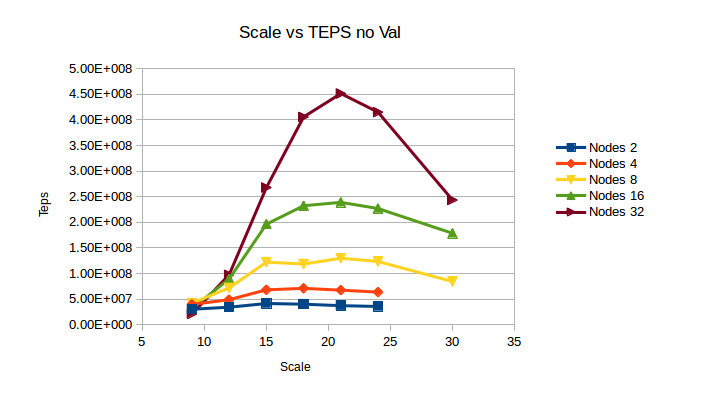
\includegraphics[width=\linewidth]{images/nodes_no_val.png}
  \caption{TEPS as a function of nodes for different scales.}
  \label{fig:nodes_no_val}
\end{subfigure}%
\begin{subfigure}{.5\textwidth}
  \centering
  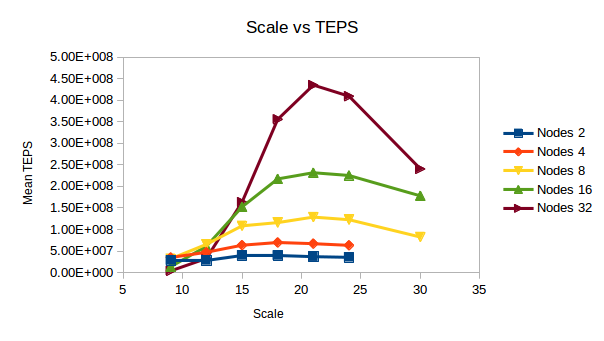
\includegraphics[width=\linewidth]{images/scale_no_val.png}
  \caption{TEPS as a function of scale for different amount of nodes.}
  \label{fig:scale_no_val}
\end{subfigure}
\caption{This figure shows the change in the amount of TEPS as a function of scale and nodes.}
\label{fig:das_no_val}
\end{figure}

\subsubsection{No InfiniBand}
The experiments on the DAS-4 have also been run without InfiniBand. The results show some similarities what has been seen previously. As before figure \ref{fig:scale_no_infini} shows an increase in TEPS as the scale increases till a certain tipping point, but unlike what has been seen in figure \ref{fig:scale_no_val} the tipping point has not been yet been reached at scale 24.
 Figure \ref{fig:nodes_no_infini} show similar results to figure \ref{fig:nodes_no_val}. The difference between the maximum TEPS for 16 nodes from the results of section \ref{res:nodes_scale} is six times as large as the maximum value for the same amount of nodes from the InfiniBand experiments.
Figure \ref{fig:scale_no_infini} also shows the same trends as figure \ref{fig:scale_no_val}. 
 
\begin{figure}[!h]
\centering
\begin{subfigure}{.5\textwidth}
  \centering
  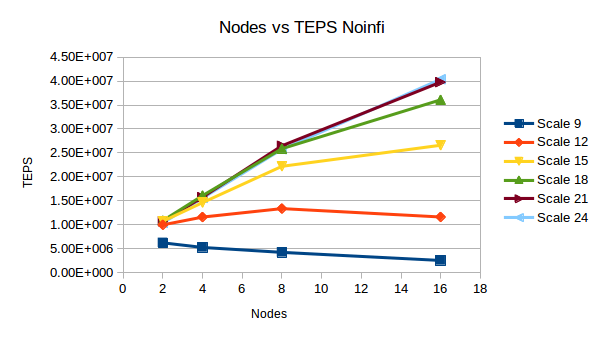
\includegraphics[width=\linewidth]{images/nodes_no_infini.png}
  \caption{TEPS as a function of nodes for different scales.}
  \label{fig:nodes_no_infini}
\end{subfigure}%
\begin{subfigure}{.5\textwidth}
  \centering
  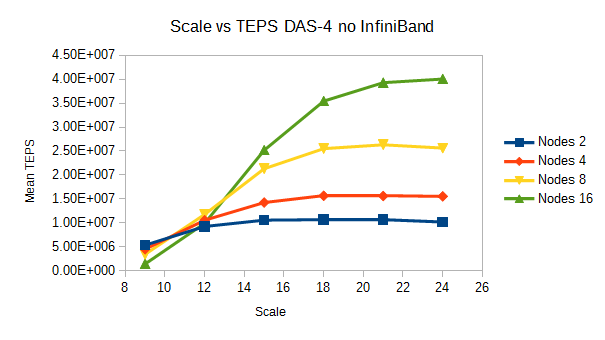
\includegraphics[width=\linewidth]{images/scale_no_infini.png}
  \caption{TEPS as a function of scale for different amount of nodes.}
  \label{fig:scale_no_infini}
\end{subfigure}
\caption{This figure shows the change in the amount of TEPS as a function of scale and nodes on the DAS-4 without using InfiniBand.}
\label{fig:das_no_infini}
\end{figure}

\subsection{OpenNebula}
The OpenNebula results can best be compared the results on the DAS-4 without InfiniBand, because the VMs on the OpenNebula do not use InfiniBand.
Looking at figure \ref{fig:das_opennebula}, the performance seems to vary significantly. The number of TEPS which can be achieved on OpenNebula is much lower than what can be seen without InfiniBand. 

The difference in performance between using four and eight nodes is much less clear on the OpenNebula, four nodes sometimes have better performance than eight nodes as seen in figure \ref{fig:nodes_opennebula}.
For the larger scales 21 and 24, the same linear correlation can be seen between the number of nodes and the performance.

The performance order of magnitude is much lower than what can be seen in Amazon and the DAS-4 without InifiBand. One of the reasons for this is the hardware it is running on. When looking at table \ref{tab:specs-opennebula} it is clear that the clock speed is lower than the other machines. Also the communication time in the OpenNebula cluster \ref{tab:imb_bench} is more than twice as long as the communication time within Amazon EC2 and about four times as long as for the DAS-4 without InfiniBand. Furthermore, the fact that there are only eight physical machines hosting all the nodes may play a part in the performance. By looking at \ref{fig:scale_opennebula} the tipping points are harder to distinguish but for four and eight nodes it can be found at scale 18. For the experiments on the DAS-4 can be found a bit later around the 18-21 point.


\begin{figure}[!h]
\centering
\begin{subfigure}{.5\textwidth}
  \centering
  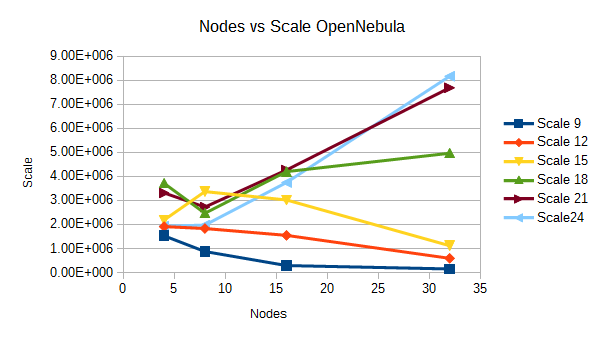
\includegraphics[width=\linewidth]{images/nodes_opennebula.png}
  \caption{TEPS as a function of nodes for different scales.}
  \label{fig:nodes_opennebula}
\end{subfigure}%
\begin{subfigure}{.5\textwidth}
  \centering
  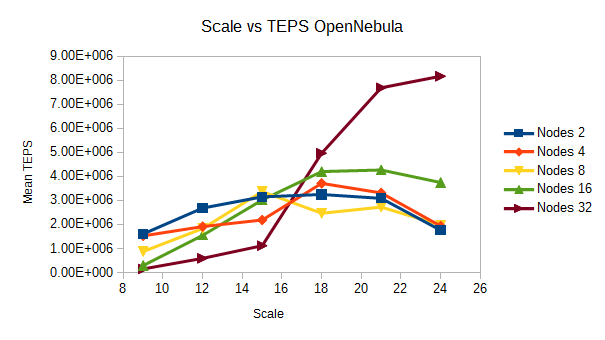
\includegraphics[width=\linewidth]{images/scale_opennebula.png}
  \caption{TEPS as a function of scale for different amount of nodes.}
  \label{fig:scale_opennebula}
\end{subfigure}
\caption{TEPS vs the scale and nodes for the experiments done on OpenNebula of the DAS-4. }
\label{fig:das_opennebula}
\end{figure}

\subsection{Amazon}
\label{res:amazon}
The figure \ref{fig:c3_amazon} and \ref{fig:r3_amazon} the results are shown for the experiments done on Amazon. The experiments have been done for two types of machines. Figure \ref{fig:c3_amazon} and \ref{fig:r3_amazon} are almost identical in terms of performance and behavior, but the r3.large can run experiments with a higher scale. The experiments done with the c3.large show that the c3.large reaches linear behavior faster than the r3.large which can be seen in figure \ref{fig:nodes_c3_amazon} and \ref{fig:nodes_r3_amazon}. For the c3.large scale 18 already shows linear behavior where as r3.large this starts at scale 21. All lines above scale 18 tightly packed on each other, as seen in figure \ref{fig:nodes_c3_amazon}.
 For the results of the r3 machines figure \ref{fig:nodes_r3_amazon} shows a more discrepancies between the scales 18 and higher. The thing to notice is that by doubling the amount of nodes used the performance also doubles.
 
Both figures show that for scales lower than 15 a different behavior is seen than for scales. At the lower scales the performance is almost constant for each number of nodes that have been tested. These scale have a tipping point at which adding more nodes only decreases the performance. 

Comparing these results with the results of the OpenNebula and the DAS-4 without InfiniBand, the AWS experiment can traverse about ten times as much edges comparing to OpenNebula. The AWS has about 50\% less TEPS than DAS-4 without Infiniband, but the behavior seen for larger scales.

 Both figures show a slow decline in performance after the tipping point in figure \ref{fig:scale_c3_amazon} and \ref{fig:scale_r3_amazon}. The parallelism becomes saturated at an earlier point for the Amazon EC2 instances than for the DAS-4. With the Amazon instances it happens at about scale 18 and for the DAS-4 18 and higher scales. Also when looking at the figures \ref{fig:nodes_c3_amazon} and \ref{fig:nodes_r3_amazon} the tipping point has not been reached for scales above 15. The behavior for smaller scales is most likely due to the communication time. As shown in table \ref{tab:imb_bench} the time taken to send messages on Amazon EC2 is twice as long compared to the DAS-4 no InfiniBand. While looking at the OpenNebula results where the communication is even longer than for EC2 the constant performance for each number of nodes is still seen up to scale 18.

\begin{figure}[!h]
	\centering
	\begin{subfigure}{.5\textwidth}
		\centering
		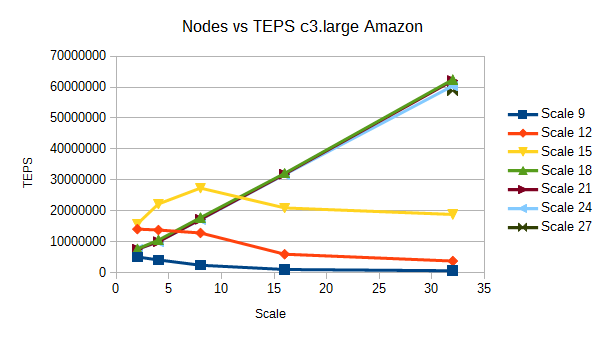
\includegraphics[width=\linewidth]{images/nodes_c3_amazon.png}
		\caption{TEPS as a function of nodes for different scales.}
		\label{fig:nodes_c3_amazon}
	\end{subfigure}%
	\begin{subfigure}{.5\textwidth}
		\centering
		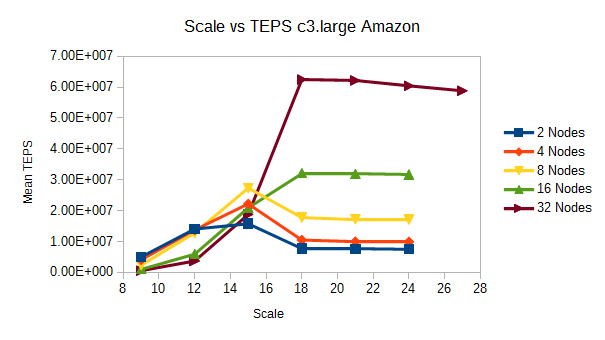
\includegraphics[width=\linewidth]{images/scale_c3_amazon.png}
		\caption{TEPS as a function of scale for different amount of nodes.}
		\label{fig:scale_c3_amazon}
	\end{subfigure}
	\caption{This figure shows the TEPS vs the scale and nodes for the experiments done on AWS c3.large machines}
	\label{fig:c3_amazon}
\end{figure}

\begin{figure}[!h]
	\centering
	\begin{subfigure}{.5\textwidth}
		\centering
		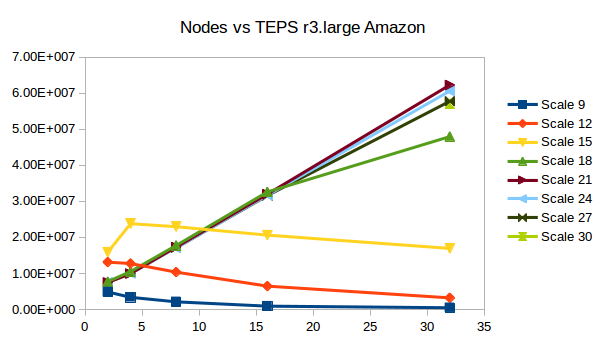
\includegraphics[width=\linewidth]{images/nodes_r3_amazon.png}
		\caption{TEPS as a function of nodes for different scales.}
		\label{fig:nodes_r3_amazon}
	\end{subfigure}%
	\begin{subfigure}{.5\textwidth}
		\centering
		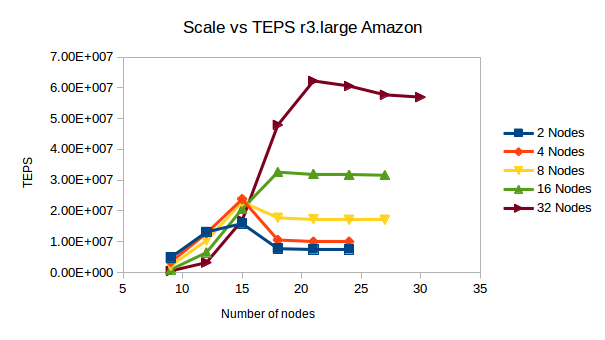
\includegraphics[width=\linewidth]{images/scale_r3_amazon.png}
		\caption{TEPS as a function of scale for different amount of nodes.}
		\label{fig:scale_r3_amazon}
	\end{subfigure}
	\caption{This figure shows the TEPS vs the scale and nodes for the experiments done on AWS r3.large machines}
	\label{fig:r3_amazon}
\end{figure}


